\documentclass[a4paper,11pt]{article}
\usepackage[T1]{fontenc}
\usepackage[utf8]{inputenc}

\usepackage[big]{layaureo}
\usepackage{amssymb,amsmath,amsthm,amsfonts,mathtools}
\usepackage{booktabs}
\usepackage{multirow}
\usepackage{siunitx}
\usepackage{graphicx}
\usepackage{caption}
\usepackage{subfig}

\usepackage{newpxtext,newpxmath}

\usepackage{float}
\floatstyle{plaintop}
\newfloat{alg}{tbp}{loc}
\floatname{alg}{Algorithm}

\usepackage{quoting}
\quotingsetup{font=small}

\usepackage[autostyle,italian=guillemets]{csquotes}
\usepackage[backend=biber]{biblatex}
\addbibresource{bib.bib}

\usepackage{tikz}
\usetikzlibrary{hobby,patterns}

\theoremstyle{definition}
\newtheorem{prop}{Proposition}
\newtheorem{defi}[prop]{Definition}
\newtheorem{thm}[prop]{Theorem}
\newtheorem{cor}[prop]{Corollary}
\newtheorem{lemma}[prop]{Lemma}
\newtheorem{rmk}[prop]{Remark}
\newtheorem{codes}[prop]{Code files}
\newtheorem{ex}[prop]{Example}
\newtheorem{prob}[prop]{Problem}

\DeclareMathOperator{\cof}{cof}
\DeclareMathOperator{\diver}{div}
\DeclareMathOperator{\vol}{vol}
\DeclareMathOperator{\are}{area}
\DeclareMathOperator{\supp}{supp}
\DeclareMathOperator{\diag}{diag}
\DeclareMathOperator{\so}{SO}
\DeclareMathOperator{\tr}{tr}
\DeclareMathOperator{\essinf}{essinf}
\DeclareMathOperator{\codim}{codim}
\DeclareMathOperator{\Iso}{Iso}

\DeclarePairedDelimiter{\norm}{\lVert}{\rVert}
\DeclarePairedDelimiter{\dual}{\langle}{\rangle}

\newcommand{\dind}[2]{\frac{\partial #1}{\partial #2}}

\newcommand{\omissis}{[\textellipsis\unkern]}

\begin{document}

\author{Bernardo Ardini [2146900]}
\date{Padova, 31 maggio 2025}
\title{\bfseries The application of bifurcation theory to the buckling of nonlinear elastic structures}

\maketitle

\begin{abstract}
This short account deal with the mathematical problems related to the study of the buckling on nonlinear elastic structures. This phenomenon occurs when an elastic structure, which is typically slender, subject to an increasing external load suddenly loses its stability.

The mathematical description of buckling is based on bifurcation theory. Most of the mechanical models used in practice are continuous models, meaning that results valid in infinite dimensional spaces, in particular Banach spaces, are required.

This work is organized as follows. In Section~\ref{sec:basics} is presented the notation that will be used. In Section~\ref{sec:preliminary} are collected some classical facts on Banach spaces. A brief outline of bifurcation theory in Banach spaces is in Section~\ref{sec:bifurcation}. In particular the Crandall-Rabinowitz theorem is proved. Starting from this theorem, in Section~\ref{sec:general-buckling} we develop a general theory for treating the buckling of nonlinear elastic structures. It is an attempt to make rigorous the heuristic considerations made in~\cite{casciaro}. In Section~\ref{sec:euler-beam} we show how to apply the general theory to a classical problem in Structural Mechanics, namely the buckling of Euler beam. Lastly, in Section~\ref{sec:body}, we describe our efforts, far to be successful, to apply the general theory of elastic buckling to the model of nonlinear hyperelastic continuous bodies. In the same Section we also treat the finite element discretization of the problem and we provide some concrete examples.
\end{abstract}

\tableofcontents

\section{Notation and basic notions}
\label{sec:basics}

\paragraph{Operators in Banach spaces} Given two Banach space $X$ and $E$ we denote by $\mathscr{L}(X,E)$ the set of linear and continuous maps from $X$ into $E$. The set of compact linear maps from $X$ into $E$ is denoted by $\mathscr{K}(X,E)$. Given $A\in\mathscr{L}(X,E)$ we call $N(A)$ and $R(A)$ its null-space and range respectively. We say that $A\in\text{Iso}(X,E)$ if $N(A)=\{0\}$ and $R(A)=E$. By closed graph theorem this implies that $A^{-1}\in\mathscr{L}(E,X)$.

\paragraph{Duality} The symbol $(\cdot,\cdot)$ always denotes the inner product in $L^2$. The duality between a Banach space $V$ and its dual $V'$ is denoted by $\dual{f,v}$ for $v\in V$ and $f\in V'$. Sometimes we will write simply $fv$ instead. In particular if $L\in\mathscr{L}(V,V')$ then $Lvw=\dual{Lv,w}$ for $v,w\in V$. We will use also notations like $Lv^2=Lvv$ for $v\in V$.

\paragraph{Fréchet derivatives} Given a $C^1$ map $F$ from an open subset $U$ of Banach space $X$ into another Banach space $E$, its Fréchet derivative is a map $DF=F'\in C^0(U,\mathscr{L}(X,E))$. In particular if $\Phi$ is a $C^2$ map from a Banach space $V$ into $\mathbb{R}$, its Fréchet derivative is a map $\Phi'\in C^1(V,V')$. The double Fréchet derivative is a map $\Phi''\in C^0(V,\mathscr{L}(V,V'))$. By Schwartz theorem $\Phi''(u)vw=\Phi''(u)wv$ for all $u\in V$ and $v,w\in V$. Similar considerations holds for higher order Fréchet derivatives.

\section{Preliminary results}
\label{sec:preliminary}

In this Section are collected some results on Banach spaces that will be useful later.

\subsection{Orthogonal spaces}

Let $V$ be Banach space.

\begin{defi}
If $N\subset V$ and $R\subset V'$ are linear subspaces, we define their orthogonal spaces as
\[
N^\perp=\{f\in V'\;|\;\dual{f,v}=0\;\forall v\in N\}
\quad\text{and}\quad
R^\perp=\{v\in V\;|\;\dual{f,v}=0\;\forall f\in R\}.
\]
\end{defi}
\begin{rmk}
It is clear that $N^\perp$ and $R^\perp$ are closed respectively in $V'$ and $V$.
\end{rmk}

\begin{prop}
\label{prop:double-orth}
If $N\subset V$ and $R\subset V'$ are linear subspaces then $(N^\perp)^\perp=\overline{N}$ and $(R^\perp)^\perp\supset\overline{R}$. Moreover if $V$ is reflexive then $(R^\perp)^\perp=\overline{R}$
\end{prop}
\begin{proof}
It is obvious that $(N^\perp)^\perp\supset\overline{N}$ and $(R^\perp)^\perp\supset\overline{R}$.

By contradiction let $v_0\in(N^\perp)^\perp$ such that $v_0\notin\overline{N}$. Then by Hahn--Banach $\{v_0\}$ and $\overline{N}$ are strictly separated, so there exists $f\in V'$ and $\alpha\in\mathbb{R}$ such that
\[
\dual{f,v}<\alpha<\dual{f,v_0}\quad\text{for all $v\in N$}.
\]
Since $N$ is a linear subspace, $\dual{f,v}=0$ for all $v\in N$ meaning that $f\in N^\perp$. In particular $\dual{f,v_0}=0$. This a contradiction.

Now assume that $V$ is reflexive. By contradiction let $f_0\in(R^\perp)^\perp$ such that $f_0\notin\overline{R}$. Then by Hahn-Banach $\{f_0\}$ and $\overline{R}$ are strictly separated, so there exists $\xi\in V''$ and $\alpha\in\mathbb{R}$ such that
\[
\dual{\xi,f}<\alpha<\dual{\xi,f_0}\quad\text{for all $f\in R$}.
\]
Since $R$ is a linear subspace, $\dual{\xi,f}=0$ for all $f\in R$. Then it must be $\dual{\xi,f_0}>0$. Since $V$ is reflexive there exists $v\in V$ such that $\dual{\xi,f}=\dual{f,v}$ for all $f\in V'$. Then $v\in R^\perp$ so $\dual{\xi,f_0}=\dual{f_0,v}=0$. Contradiction.
\end{proof}

\subsection{Self-adjoint operators}

Let $V$ be a reflexive Banach space and $L\in\mathscr{L}(V,V')$.

\begin{defi}
We say that $L$ is self-adjoint if $\dual{Lv,w}=\dual{Lw,v}$ for all $v,w\in V$.
\end{defi}

\begin{prop}
\label{prop:range-adj}
If $L$ is self-adjoint and $R(L)$ is closed then $R(L)=N(L)^\perp$.
\end{prop}
\begin{proof}
% my proof
First we show that $R(L)^\perp=N(L)$. Indeed $w\in R(L)^\perp$ if and only if $\dual{Lv,w}=\dual{Lw,v}=0$ for all $v\in V$ and this is equivalent to $Lw=0$.

Then $(R(L)^\perp)^\perp=N(L)^\perp$ and the thesis follows by Proposition~\ref{prop:double-orth} and the fact that $R(L)$ is closed.
\end{proof}

\subsection{Complemented spaces and codimension}

Let $E$ be a Banach space.
\begin{defi}
A closed subspace $R$ of $E$ is complemented if there exists a closed complement $C$, i.e., a closed subspace of $E$ such that $E=R\oplus C$. The codimension of $R$ is the dimension of $C$ (it is obvious that it does not depend on $C$).
\end{defi}
\begin{rmk}
Every finite dimensional space $R$ is complemented. Indeed take a basis $\{f_i\}_{i=1}^n$ of $R$ and consider the functionals $\xi_i\in R'$ that send an $f\in R$ into its components along vector $f_i$. Then extend $\xi_i$ as a functional in $E'$ by Hahn--Banach theorem. Now a complement of $R$ is simply
\[
C=\{f\in E\;|\;\dual{\xi_i,f}=0\quad\forall i=1,\dots,n\}.
\]
Indeed every $f\in E$ decompose uniquely as $f=\sum_{i=1}^n\dual{\xi_i,f}f_i+(f-\sum_{i=1}^n\dual{\xi_i,f}f_i)$.
\end{rmk}

We give below a necessary and sufficient condition for $R$ to be complemented and of finite codimension.
\begin{prop}
\label{prop:codim}
Let $R$ be a closed subspace of $E$. Then $R$ is complemented and of finite codimension $n$ if and only if there exist $\{\xi_i\}_{i=1}^n\subset E'$ linearly independent such that
\begin{equation}
\label{eqn:annihilated}
R=\{f\in E\;|\;\dual{\xi_i,f}=0\quad\forall i=1,\dots,n\}.
\end{equation}
\end{prop}
\begin{proof}
% my proof
Assume that $R$ has a complement $C$ of finite dimension $n$. Let $\{f_i\}_{i=1}^n$ be a basis of $C$. Now given any $f\in E$, decompose it uniquely as $f=r+c$, where $r\in R$ and $c=\sum_{i=1}^{n}c_if_i\in C$. We define $\{\xi_i\}_{i=1}^n\subset E'$ by $\dual{\xi_i,f}=c_i$. It is clear that~\eqref{eqn:annihilated} holds.

Conversely assume that there exist $\{\xi_i\}_{i=1}^n$ such that~\eqref{eqn:annihilated} holds. Then let $f_1\in E$ such that $\dual{\xi_1,f_1}=1$. Define
\[
R_1=\{f\in E\;|\;\dual{\xi_1,f}=0\}\quad\text{and}\quad C_1=\text{span}(f_1).
\]
It is clear that $E=R_1\oplus C_1$. Indeed given $f\in E$ we write it uniquely as $f=(f-\dual{\xi_1,f}f_1)+\dual{\xi_1,f}f_1$. Now define $\tilde{\xi}_2=\xi_2-\dual{\xi_2,f_1}\xi_1$ so that $\dual{\tilde{\xi}_2,f_1}=0$. Let $f_2\in R_1$ such that $\dual{\tilde\xi_2,f_2}=1$. If we set
\[
R_2=\{f\in E\;|\;\text{$\dual{\xi_1,f}=0$ and $\dual{\tilde{\xi}_2,f}=0$}\}\quad\text{and}\quad C_2=\text{span}(f_1,f_2),
\]
it is easy to prove that $E=R_2\oplus C_2$. By induction we construct $\{\tilde\xi_i\}_{i=1}^n$, with $\tilde\xi_1=\xi_1$, and $\{f_i\}_{i=1}^n$ such that if
\[
R_n=\{f\in E\;|\;\dual{\tilde\xi_i,f}=0\quad\forall i=1,\dots,n\}.\quad\text{and}\quad C_n=\text{span}(\{f_i\}_{i=1}^n),
\]
then $E=R_n\oplus C_n$. The span of $\{\tilde\xi_i\}_{i=1}^n$ coincides with the span of $(\{\xi_i\}_{i=1}^n)$ so $R=R_n$. Moreover $\{f_i\}_{i=1}^n$ are linearly independent, so $C=C_n$ is a complement of $R$ of dimension $n$.
\end{proof}

We get the following corollary that relates the dimension of the nullspace of an adjoint operator with the codimension of its range.
\begin{cor}
Let $V$ a reflexive Banach space and $L\in\mathscr{L}(V,V')$ a self-adjoint operator with $R(L)$ closed and $N(L)$ of finite dimension. Then $R(L)$ is complemented and $\codim(R(L))=\dim(N(L))$.
\end{cor}
\begin{proof}
Let $\{v_i\}_{i=1}^n$ be a basis of $N(L)$. Since $V$ is reflexive there exist unique $\{\xi_i\}_{i=1}^n\subset V''$ such that $\dual{\xi_i,f}=\dual{f,v_i}$ for any $f\in V'$. By Proposition~\ref{prop:range-adj} we have that
\[
R(L)=N(L)^\perp=\{f\in V'\;|\;\dual{\xi_i,f}=0\quad\forall i=1,\dots,n\}.
\]
The thesis follows by Proposition~\ref{prop:codim}.
\end{proof}

\section{Bifurcation theory in Banach spaces}
\label{sec:bifurcation}

Let $X$ and $E$ be Banach spaces. Consider a map $F$ of class $C^r$, with $r\ge1$, from a neighborhood of $x_0\in X$ into $E$ such that $F(x_0)=0$. We are concerned with the equation
\[
F(x)=0
\]
when $x$ is near $x_0$. By making a change of variable we can always assume that $x_0=0$. When the Inverse Function Theorem applies the set of solutions around the origin is a regular manifold. When it does not apply it can be more complicated and bifurcations can occur.

In this Section we first recall the Implicit Function Theorem. Then we present the Lyapunov-Schmidt procedure, a tool allowing us to reduce the study of the set of solutions to the equation $F(x)=0$ to a simpler problem involving only finite dimensional spaces. Then we will prove a theorem of Crandall and Rabinowitz that gives sufficient conditions for the existence of a bifurcation. All the results of this Section are taken from~\cite{niremberg}.

\subsection{The Implicit Function Theorem}

The following theorem is a well known form of the Implicit Function Theorem.
\begin{thm}
\label{thm:IFT}
Let $V$, $\Lambda$ and $E$ be Banach spaces. Let $F=F(u,\lambda)$ be a $C^r$ map, with $r\ge1$, from a neighborhood of $(u_0,\lambda_0)\in V\times\Lambda$ into $E$ such that $F(u_0,\lambda_0)=0$ and $D_uF(u_0,\lambda_0)\in\text{Iso}(V,E)$. Then there exists a $C^r$ map $\upsilon$ from a neighborhood of $\lambda_0$ into $V$ such that $\upsilon(\lambda_0)=u_0$ and locally around $(u_0,\lambda_0)$ the solutions $(u,\lambda)$ to $F(u,\lambda)=0$ satisfies $u=\upsilon(\lambda)$.
\end{thm}

We report below an alternative form of the Implicit Function Theorem which is more suitable for treating the problem described at the beginning of this Section.
\begin{cor}
\label{cor:alt-IFT}
Let $X$ and $E$ be a Banach spaces and $U\subset X$ open. Let $F\in C^r(U,E)$ with $r\ge1$. Let $0\in U$ and assume that
\begin{itemize}
\item[(i)] $F(0)=0$,
\item[(ii)] $N(DF(0))=X_1$ has a complement $X_2$,
\item[(iii)] $R(DF(0))=E$.
\end{itemize}
Then there exists $\delta>0$ such that for all $x_1\in X_1$ with $\norm{x_1}\le\delta$ there exists a unique $x_2=\chi(x_1)\in X_2$ such that
\[
F(x_1+x_2)=0.
\]
Moreover $\chi(0)=0$ and $\chi$ is a $C^r$ map from $B(0,\delta)\subset X_1$ into $X_2$.
\end{cor}
\begin{proof}
Define $G(x_2,x_1)=F(x_1+x_2)$ for $x_1\in X_1$ and $x_2\in X_2$ with $x_1+x_2\in U$. The map $G$ is from a neighborhood of $(0,0)$ in $X_2\times X_1$ into $E$. By (i) we have $G(0,0)=0$. Moreover $D_{x_2}G(0,0)=DF(0,0)\in\text{Iso}(X_2,E)$ because of (ii) and (iii).

Then by Theorem~\ref{thm:IFT} with $X_2$ and $X_1$ instead of $V$ and $\Lambda$ respectively, we have the thesis.
\end{proof}

\subsection{The Lyapunov--Schmidt procedure}

Let $X$ and $E$ be Banach spaces and $F$ a map of class $C^r$, with $r\ge1$, from a neighborhood of the origin in $X$ into $E$ such that $F(0)=0$. Assume that $DF(0)$ is Fredholm, i.e.,
\begin{itemize}
\item[(a)] $N(DF(0))=X_1$ has finite dimension $n$ and
\item[(b)] $R(DF(0))=E_1$ is a closed subspace of finite codimension.
\end{itemize}
Let $X_2$ and $E_2$ some complements of $X_1$ and $E_1$ respectively. Then consider the projection $Q$ into $E_1$ associated to the decomposition $E=E_1\oplus E_2$. Now equation $F(x)=0$ can be written as
\[
QF(x)=0\quad\text{and}\quad (I-Q)F(x)=0.
\]
Let $x\mapsto QF(x)$ be defined in a neighborhood of $0$ into $E_1$. Now by applying Corollary~\ref{cor:alt-IFT} to it we have that there exists $\chi$ of class $C^r$ from a neighborhood of the origin in $X_1$ into $X_2$ such that $\chi(0)=0$ and
\[
QF(x_1+\chi(x_1))=0.
\]
Then it remains only to solve the following \emph{bifurcation equation}:
\begin{equation}
\label{eqn:finite-dim}
(I-Q)F(x_1+\chi(x_1))=0\quad\text{for $x_1\in X_1$ near the origin}.
\end{equation}
Since $X_1$ and $E_2$ are finite dimensional it is a fully finite dimensional problem.

If $E_1=E$ then $E_2=0$ and equation~\eqref{eqn:finite-dim} is trivially satisfied. In this case the solutions of $F(x)=0$ around 0 are of the form $x_1+\chi(x_1)$ so they form a $C^r$ manifold of dimension $n$.

When $R(DF(0))\neq E$ bifurcations can occur. We confine ourself with the case in which $\codim(E_1)=\dim(E_2)=1$. In this case equation~\eqref{eqn:finite-dim} is actually a scalar equation. Indeed by Proposition~\ref{prop:codim} there exists $\xi\in E'$ such that $E_1=\{f\in E\;|\;\dual{\xi,f}=0\}$, so the bifurcation equation can be rewritten as
\[
G(x_1):=\dual{\xi,F(x_1+\chi(x_1))}=0.
\]
By choosing a basis in $X_1$, the function $G$ can be understood as a function from a neighborhood of the origin in $\mathbb{R}^n$ into $\mathbb{R}$.

\subsection{A local bifurcation theorem of Crandall and Rabinowitz}

We now want to understand under which conditions from equation $G(x_1)=0$ arise a bifurcation. The following result will be useful.
\begin{lemma}[Morse lemma]
Let $G$ a $C^r$ map, with $r\ge2$, from a neighborhood of the origin in $\mathbb{R}^n$ into $\mathbb{R}$. Assume that
\begin{itemize}
\item[(i)] $G(0)=0$,
\item[(ii)] $DG(0)=0$ and
\item[(iii)] $D^2G(0)$ is a nonsingular $n$-by-$n$ matrix.
\end{itemize}
Then there exists a $C^{r-2}$ change of variable $y=y(x)$ around the origin such that $y(0)=0$ and
\[
G(x)=\frac{1}{2}y(x)^TD^2G(0)y(x).
\]
Moreover if $r\ge3$ then $Dy(0)=I$.
\end{lemma}
We get immediately the following corollary.
\begin{cor}
\label{cor:cor-morse}
Assume that the hypotheses of Morse lemma holds. Assume also that $n=2$ and that $D^2G(0)$ is indefinite. Then the set of solutions of the equation $G(x)=0$ near the origin is made by two $C^{r-2}$ curves intersecting only at the origin. Moreover if $r\ge3$ they intersect transversally.
\end{cor}
\begin{proof}
The equation $\frac{1}{2}y^TD^2G(0)y$ admits as a solution set two distinct lines intersecting at the origin. Indeed we can assume that
\[
D^2G(0)=
\begin{pmatrix}
\frac{1}{a_1^2} & 0 \\
0 & -\frac{1}{a_2^2}
\end{pmatrix}
\]
so we have
\[
\frac{y_1^2}{a_1^2}-\frac{y_2^2}{a_2^2}=0
\]
which is exactly the equation of two lines intersecting at the origin.

Applying the change of variable, we find that the set of solutions to $G(x)=0$ around the origin is a deformation of these two lines. When $r\ge3$ then the change of variable is at least $C^1$ and the Jacobian matrix is the identity at the origin so the two curves still intersect transversally.
\end{proof}
Now we can obtain the main result of this Section.
\begin{thm}[Crandall and Rabinowitz]
\label{thm:gen-bif}
Let $X$ and $E$ be Banach spaces and $F$ a map of class $C^r$, with $r\ge2$, from a neighborhood of the origin in $X$ into $E$ such that $F(0)=0$. Assume that
\begin{itemize}
\item [(i)] $N(DF(0))$ has dimension 2 and
\item[(ii)] $R(DF(0))$ is closed and has codimension 1.
\end{itemize}
Let $\xi\in E'$ such that $R(DF(0))=\{f\in E\;|\;\dual{\xi,f}=0\}$. Define a 2-by-2 matrix $M$ as the Hessian of the map
\begin{align*}
N(DF(0))\to\mathbb{R} \\
x\mapsto\dual{\xi,F(x)},
\end{align*}
computed at the origin and expressed with respect to some basis in $N(DF(0))$. If $M$ is nonsingular and indefinite then the set of solution to $F(x)=0$ near the origin is made of two $C^{r-2}$ curves intersecting only at the origin. If $r\ge3$ then they intersect transversally.
\end{thm}
\begin{proof}
We have only to show that $DG(0)=0$ and $D^2G(0)=M$. Indeed by applying Corollary~\ref{cor:cor-morse} we would get the thesis.

\emph{Step 1.} For $v\in N(DF(0))$
\[
DG(x)v=\dual{\xi,DF(x+\chi(x))(v+D\chi(x)v)}\quad\text{so}\quad DG(0)v=\dual{\xi,DF(0)(v+D\chi(0)v)}=0,
\]
where last equality holds by definition of $\xi$.

\emph{Step 2.} From
\[
F(x+\chi(x))=0\quad\text{when $x\in N(DF(0))$ is near 0},
\]
we get by differentiating that
\[
DF(0)v+DF(0)D\chi(0)v=0
\]
for all $v\in N(DF(0))$. But $DF(0)v=0$ so $DF(0)D\chi(0)v=0$. It follows that $D\chi(0)v\in N(DF(0))\cap X_2$ so $D\chi(0)=0$.

\emph{Step 3.} For $v,w\in N(DF(0))$ we have
\begin{align*}
D^2G(0)vw&=\dual{\xi,D^2F(0)(v+D\chi(0)v)(w+D\chi(0)w)}+\dual{\xi,DF(0)D^2\chi(0)vw}=\\
&=\dual{\xi,D^2F(0)vw}=Mv\cdot w.
\end{align*}
where we have used the definition of $\xi$ and the previous step to say that $D\chi(0)=0$. 
\end{proof}

\section{Buckling of general nonlinear elastic structures}
\label{sec:general-buckling}

Consider an elastic structure whose kinematically admissible configurations are described by the elements $u$ of a reflexive Banach space $V$. Assume that the energy of the structure comprehensive of both the elastic energy and the energy of the loads is
\[
\Pi\in C^{r+1}(V\times\mathbb{R})\quad\text{with $r\ge2$},\qquad(u,\lambda)\mapsto\Pi(u,\lambda),
\]
where $\lambda\in\mathbb{R}$ describes the intensity of the loads. We will see examples of such structures in the following sections.

\begin{rmk}
In what follows we will denote by $\cdot'$ the Fréchet derivatives with respect to $u$ and by $\hat{\cdot}$ the derivatives with respect to $\lambda$. The Fréchet derivative with respect to $(u,\lambda)$ is denoted by $D\cdot$.
\end{rmk}

The out of balance force acting on the structure is defined as $F=\Pi'\in C^2(V\times\mathbb{R},V')$. Hence we say that $u\in V$ is an equilibrium configuration corresponding to a load $\lambda\in\mathbb{R}$ if $F(u,\lambda)=0$. We are interested in the study of the solution set of the equilibrium equation
\[
F(u,\lambda)=0.
\]

\begin{rmk}
\label{rmk:adj}
By Schwartz theorem $F'(u,\lambda)=\Pi''(u,\lambda)$ is a self-adjoint operator in $\mathscr{L}(V,V')$ for all $(u,\lambda)\in V\times\mathbb{R}$. Indeed $\Pi''(u,\lambda)vw=\Pi''(u,\lambda)wv$ for $v,w\in V$. Moreover in concrete problems it happens that $R(F'(u,\lambda))$ is closed for all $(u,\lambda)\in V\times\mathbb{R}$. Then by Proposition~\ref{prop:range-adj} we have $R(F'(u,\lambda))=N(F'(u,\lambda))^\perp$.
\end{rmk}

\subsection{Critical points}
\label{subsec:critical-points}

Let $(u_0,\lambda_0)\in V\times\mathbb{R}$ such that $N(F'(u_0,\lambda_0)))=\{0\}$. Then by Remark~\ref{rmk:adj} we have that $R(F'(u_0,\lambda_0))=V'$. This means that $F'(u_0,\lambda_0)\in\text{Iso}(V,V')$. By the Implicit Function Theorem then the solutions near $(u_0,\lambda_0)$ lies on a curve of the form $\lambda\mapsto(u(\lambda),\lambda)$ where $u$ is a $C^2$ map defined in a neighborhood of $\lambda_0$ into $V$.

The structure of the solution set can be more complicated near a critical point.
\begin{defi}
A point $(u_c,\lambda_c)\in V\times\mathbb{R}$ is called a \emph{critical point} if $N(F'(u_c,\lambda_c))\neq\{0\}$.
\end{defi}
\begin{rmk}
For simplify the notation we will simply write a subscript $c$ to denote quantities computed at $(u_c,\lambda_c)$.
\end{rmk}
We will confine ourself to the case in which $N(F_c')=\text{span}(v_c)$ has dimension one. In this case we distinguish two different types of critical points.

\paragraph{Limit points} If $\hat{F}_cv_c\neq0$ then $(\lambda_c,u_c)$ is called a \emph{limit point}. Suppose there exists a $C^1$ curve of solutions $t\mapsto(u(t),\lambda(t))$ defined in a neighborhood of $t=0$ such that $(u_0,\lambda_0)=(u_c,\lambda_c)$. (We mark with a 0 subscript quantities computed at $t=0$). From $0=F(u,\lambda)$, by differentiating with respect to $t$ we get
\begin{equation}
\label{eqn:eq-diff}
0=F'_c\dot u_0+\dot\lambda_0\hat{F}_c.
\end{equation}
Acting with this equality on $v_c$ and using that $F_c'$ is self-adjoint we have
\[
0=F'_c\dot u_0v_c+\dot\lambda_0\hat{F}_cv_c=F'_cv_c\dot u_0+\dot\lambda_0\hat{F}_cv_c=\dot\lambda_0\hat{F}_cv_c.
\]
Since $\hat{F}_cv_c\neq0$ it follows that $\dot\lambda_0=0$ and substituting back into~\eqref{eqn:eq-diff} we have $\dot u_0\in N(F_c')$. The typical situation is depicted in Figure~\ref{fig:critical-points}~(a).
\begin{rmk}
Clearly there can be more then one curve passing through $(u_c,\lambda_c)$. In this case all this curves would intersect tangentially, but $(u_c,\lambda_c)$ would not be a limit point but actually a bifurcation point. See Figure~\ref{fig:critical-points}~(b). Anyway we will not deal with such situation.
\end{rmk}

\begin{figure}[t]
\centering
\footnotesize

\subfloat[][]
{
\begin{tikzpicture}
\draw (-0.3,0) -- (3,0);
\draw (0,-0.3) -- (0,3);
\draw [use Hobby shortcut] (0.5,0.5)..(0.6,1)..(2,1.1)..(1.7,2);
\draw[fill=black] (2.2,1.5) circle (0.03);
\node[anchor=west] at (2.2,1.5) {$(u_c,\lambda_c)$};
\node[anchor=west] at (3,0) {$\lambda$};
\node[anchor=south] at (0,3) {$u$};
\end{tikzpicture}
}
\quad
\subfloat[][]
{
\begin{tikzpicture}
\draw (-0.3,0) -- (3,0);
\draw (0,-0.3) -- (0,3);
\draw [use Hobby shortcut] (0.2,0.5)..(0.4,1)..(0.9,1.1)..(0.7,2);
\draw [use Hobby shortcut] (2,0.3)..(1.2,1)..(1.4,2)..(1.7,2.3);
\draw[fill=black] (1.17,1.46) circle (0.03);
\node[anchor=west] at (1.17,1.46) {$(u_c,\lambda_c)$};
\node[anchor=west] at (3,0) {$\lambda$};
\node[anchor=south] at (0,3) {$u$};
\end{tikzpicture}
}
\quad
\subfloat[][]
{
\begin{tikzpicture}
\draw (-0.3,0) -- (3,0);
\draw (0,-0.3) -- (0,3);
\draw [use Hobby shortcut] (0.2,0.8)..(0.6,1)..(2,1.1)..(2.2,1.2);
\draw [use Hobby shortcut] (0.3,0.2)..(0.7,0.4)..(2,1.8)..(2.2,2);
\draw[fill=black] (1.37,1.04) circle (0.03);
\node[anchor=north west] at (1.37,1.04) {$(u_c,\lambda_c)$};
\node[anchor=west] at (3,0) {$\lambda$};
\node[anchor=south] at (0,3) {$u$};
\end{tikzpicture}
}

\caption{Examples of critical points.}
\label{fig:critical-points}
\end{figure}

\paragraph{Bifurcation points} If $\hat{F}_cv_c=0$ then $(\lambda_c,u_c)$ is called a \emph{bifurcation point}. To motivate such denomination lets argue as follows.

\emph{Step 1.} Assume there exists a $C^2$ curve $\lambda\mapsto(u^*(\lambda),\lambda)$ defined in a neighborhood of $\lambda_c$ and passing through $(u_c,\lambda_c)$. We refer to it as the fundamental path.

\emph{Step 2.} We look for others $C^2$ curves of solutions of the form
\[
t\mapsto(u(t),\lambda(t))=\left(u^*(\lambda(t))+w(t),\lambda(t)\right),
\]
where $\lambda_0=\lambda_c$, $w_0=0$ and $t$ lies in a neighborhood of 0.

\emph{Step 3.} By differentiating $0=F(u,\lambda)$ with respect to $t$ we have
\[
0=F_c'\dot u_0+\dot\lambda_0\hat{F}_c=\dot\lambda_0(F_c'\hat u^*_c+\hat{F}_c)+F'_c\dot w_0=F'_c\dot w_0.
\]
We used that also $(u^*,\lambda)$ is a curve of solutions. It follows that $\dot w_0=\alpha v_c$ for some $\alpha\in\mathbb{R}$.

\emph{Step 3.} Differentiating again with respect to $t$ we get
\begin{equation}
\label{eqn:second-derivative}
0=F_c'\ddot u_0+F_c''\dot u_0^2+2\dot\lambda_0\hat{F}'_c\dot u_0+\ddot\lambda_0\hat{F}_c+\dot\lambda_0^2\hat{\hat{F}}_c.
\end{equation}
We act with this equality on $v_c$ so, using $F'_cv_c=0$ and $\hat F_cv_c=0$, we have
\[
0=F_c''\dot u_0^2v_c+2\dot\lambda_0\hat{F}'_c\dot u_0v_c+\dot\lambda_0^2\hat{\hat{F}}_cv_c.
\]
Hence
\[
0=\dot\lambda_0^2(F_c''(\hat u^*_c)^2v_c+2\hat{F}'\hat u^*_cv_c+\hat{\hat{F}}_cv_c)+2\dot\lambda_0F_c''\hat u_c^*\dot{w}_0v_c+F_c''\dot w_0^2v_c+2\dot\lambda_0\hat{F}_c'\dot w_0v_c.
\]
Using that $(u^*,\lambda)$ is a curve of solutions the first term vanish and we are left with
\begin{equation}
\label{eqn:alpha-two}
0=F_c''v_c^3\alpha^2+2\dot\lambda_0(F_c''\hat u_c^*v_c^2+\hat{F}_c'v_c^2)\alpha.
\end{equation}
The solution $\alpha=0$ correspond to the fundamental path. Suppose $F_c''v_c^3\neq0$. If $F_c''\hat u_c^*v_c^2+\hat{F}_c'v_c^2=0$ then the only solution is $\alpha=0$ and no bifurcation occur. (Actually there could be a bifurcation if another curve of solution intersect the fundamental path tangentially as in Figure~\ref{fig:critical-points}~(b)). If instead $F_c''\hat u_c^*v_c^2+\hat{F}_c'v_c^2\neq0$ a solution with $\alpha\neq0$ (and $\dot\lambda_0\neq 0$) is admitted. This suggest that another curve of solutions intersect the fundamental path at $(u_c,\lambda_c)$ transversally. The situation is represented in Figure~\ref{fig:critical-points}~(c).

\subsection{A local bifurcation theorem suitable for the elastic buckling analysis}

We now want to understand under which conditions at a bifurcation point, as defined in the previous paragraph, a bifurcation actually occurs. Thanks to the insight just gained by the previous computations, we claim the following theorem. It is the main theorem of this work. We obtained the proof by generalizing that of \cite[Theorem 3.3.3]{niremberg}.

\begin{thm}
\label{thm:main}
Let $V$ be a reflexive Banach space and $F$ a $C^r$ map, with $r\ge2$, from a neighborhood of $(u_c,\lambda_c)\in V\times\mathbb{R}$ into $V'$. Suppose
\begin{itemize}
\item[(i)] $F_c=0$,
\item[(ii)] $F'_c\in\mathscr{L}(V,V')$ is self-adjoint and $R(F'_c)$ is closed,
\item[(iii)] $N(F'_c)=\text{span}(v_c)$ is one dimensional.
\end{itemize}
Suppose also that there exists $(\hat{u}^*_c,1)\in V\times\mathbb{R}$ such that
\begin{itemize}
\item[(iv)] $F'_c\hat{u}^*_c+\hat{F}_c=0$,
\item[(v)] $F_c''(\hat{u}_c^*)^2v_c+2\hat{F}_c'\hat{u}_c^*v_c+\hat{\hat{F}}_cv_c=0$ and
\item[(vi)] $F_c''\hat{u}_c^*v_c^2+\hat{F}_c'v_c^2\neq0$.
\end{itemize}

Then at $(u_c,\lambda_c)$ a bifurcation occur. In fact the set of solutions of $F(u,\lambda)=0$ near $(u_c,\lambda_c)$ consists of two $C^{r-2}$ curves intersecting only at $(u_c,\lambda_c)$. If $r\ge3$ they intersect transversally.
\end{thm}
\begin{proof}
% my proof
We want to apply Theorem~\ref{thm:gen-bif} to map $F$. The proof if complete if we verify the hypotheses of that theorem. This is done in the steps below.

\emph{Step 1.} We prove that $N(DF_c)$ is of dimension 2 and spanned by $(v_c,0)$ and $(\hat{u}^*_c,1)$. By (ii) and (iv) it is clear that these two vectors both belong to $N(DF_c)$ and are linearly independent. Let $(\dot u_0,\dot\lambda_0)\in N(DF_c)$. We need only to prove that it is a linear combination of $(v_c,0)$ and $(\hat{u}^*_c,1)$. We have
\begin{gather*}
\dot\lambda_0F_c'\hat{u}^*_c+\dot\lambda_0\hat{F}_c=0\quad\text{and}\quad F_c'\dot u_0+\dot\lambda_0\hat{F}_c=0.
\end{gather*}
By making the difference
\[
F_c'(\dot u_0-\dot\lambda_0\hat{u}^*_c)=0,
\]
so there exists $\beta\in\mathbb{R}$ such that $\dot u_0=\dot\lambda_0\hat u_c^*+\beta v_c$. Hence
\[
(\dot u_0,\dot\lambda_0)=\dot\lambda_0(\hat u_c^*,1)+\beta(v_c,0)\in\text{span}\left(\{(v_c,0),(\hat{u}^*_c,1)\}\right).
\]

\emph{Step 2.} We prove that $R(DF_c)=R(F_c')$. From this would follow that $R(DF_c)$ is closed and of codimension 1 (see Remark~\ref{rmk:adj}). The general element of $f\in R(DF_c)$ can be written as
\[
f=F_c'v+\beta\hat F_c\quad\text{for $v\in V$ and $\beta\in\mathbb{R}$}.
\]
Now from hypothesis (iv) we have that $\hat F_c=-F'_c\hat u_c^*$. This means that actually $f\in R(F_c')$.

\emph{Step 3.} From Remark~\ref*{rmk:adj} we know that
\[
R(F_c')=\{f\in V'\;|\;\dual{f,v_c}=0\}=\{f\in V'\;|\;\dual{\xi_c,f}=0\},
\]
where $\xi_c\in V''$ is the element corresponding to $v_c$. We now compute the matrix $M$ defined as the Hessian of the map
\begin{align*}
N(DF(0))&\to\mathbb{R} \\
(w,\mu)&\mapsto\dual{\xi_c,F(w,\mu)}=\dual{F(w,\mu),v_c}.
\end{align*}
By using $(v_c,0)$ and $(\hat u_c^*,1)$ as a basis of $N(DF_c)$, after some computations we get
\[
M=
\begin{pmatrix}
F_c''v_c^3 & F_c''\hat{u}_c^*v_c^2+\hat{F}_c'v_c^2 \\
F_c''\hat{u}_c^*v_c^2+\hat{F}_c'v_c^2 & F_c''(\hat{u}_c^*)^2v_c+2\hat{F}_c'\hat{u}_c^*v_c+\hat{\hat{F}}_cv_c.
\end{pmatrix}
\]
Notice that by (v) and (vi) it follows that $\det(Q)<0$. So $Q$ is nonsingular and indefinite.
\end{proof}

\begin{rmk}
In the discussion of previous Subsection we supposed that $F_c''v_c^3\neq0$. The theorem ensure the existence of a bifurcating curve intersecting transversally the fundamental path even without this additional assumption.
\end{rmk}

\subsection{Koiter asymptotic analysis}
\label{subsec:koiter}

Theorem~\ref{thm:main} make rigorous the asymptotic analysis of buckled structures introduced by Koiter~\cite{koiter} in 1942. It consists in the asymptotic approximation of the bifurcating curve near the bifurcation point. We will give now a brief description of it. In the following discussion we assume that $r\ge6$.

\paragraph{Fundamental path} Let $\lambda\mapsto(u^*(\lambda),\lambda)$ be a $C^{r-2}$ curve of solutions defined for $\lambda\in[0,\Lambda]$. We call it the \emph{fundamental path} and we assume it is known. In practice this path describes the deformation of the structure before the onset of instability, starting from its reference configuration $u=0$, when $\lambda=0$, and then increasing the load.

\paragraph{Critical load} Let $\lambda_c\in(0,\Lambda)$ be the \emph{critical load},~i.e., the smallest load such that $(u_c^*,\lambda_c)=(u_c,\lambda_c)$ is a critical point. Assume that all the hypotheses of Theorem~\ref{thm:main} are satisfied. Hence there exists a $C^{r-2}$ curve $t\mapsto(u(t),\lambda(t))$ intersecting the fundamental path transversally at $(u_c,\lambda_c)$. Assume that $(u_0,\lambda_0)=(u_c,\lambda_c)$.

\paragraph{Elastic buckling} In practice the equilibrium solutions $(u^*(\lambda),\lambda)$ for $\lambda>\lambda_c$ are unstable. This means that when the critical load is reached the fundamental path is abandoned and the equilibrium is established on the bifurcating curve which we will call \emph{buckling path}. This phenomenon is indeed called \emph{elastic buckling}.

\begin{rmk}
In this work we will not deal with the stability of elastic equilibrium so we accept the previous consideration as granted. For possible definitions of stability of elastic equilibrium see~\cite[Chapter 2]{koiter}.
\end{rmk}

\paragraph{First order approximation} The computations made in Subsection~\ref{subsec:critical-points} when the bifurcations points where introduced, are completely justified by Theorem~\ref{thm:main}. So we can write the buckling path as
\[
t\mapsto(u(t),\lambda(t))=\left(u^*(\lambda(t))+w(t),\lambda(t)\right),
\]
where $w(\cdot)$ and $\lambda(\cdot)$ are $C^{r-2}$ curves vanishing at $t=0$. We choose $\alpha=1$ so $\dot w_0=v_c$. A different choice corresponds to a different parametrization of the curve. From equation~\eqref{eqn:alpha-two} it follows that
\begin{equation}
\label{eqn:lambda-dot}
\dot\lambda_0=-\frac{1}{2}\frac{F_c''v_c^3}{F_c''\hat u_c^*v_c^2+\hat{F}_c'v_c^2}.
\end{equation}
In this way we obtain the first order approximation of the buckling path:
\begin{equation}
\label{eqn:first-order}
(u(t),\lambda(t))=(u^*(\lambda_c+\dot\lambda_0t)+v_ct,\lambda_c+\dot\lambda_0t)+\mathscr{O}(t^2).
\end{equation}

\paragraph{Second order approximation} We start from equation~\eqref{eqn:second-derivative}. Substituting onto it $\dot u_0=\dot\lambda_0\hat u^*_c+v_c$ and $\ddot u_0=\ddot\lambda_0\hat u^*_c+\dot\lambda_0^2\hat{\hat{ u}}^*_c+\ddot w_0$ we have
\[
0=\ddot\lambda_0(F_c'\hat u_c^*+\hat F_c)+\dot\lambda_0^2(F_c'\hat{\hat u}^*_c+F_c''\hat u_c^*+2F_c'\hat u_c^*+\hat{\hat F}_c)+F_c'\ddot w_0+F_c''v_c^2+2\dot\lambda_0(F_c''\hat u_c^*v_c+\hat F_c'v_c).
\]
The first two term vanish so we obtain the following equation for $\ddot w_0$:
\begin{equation}
\label{eqn:w-ddot}
F_c'\ddot w_0=-F_c''v_c^2-2\dot\lambda_0(F_c''\hat u_c^*v_c+\hat F_c'v_c).
\end{equation}
This equation does not have a unique solution since $N(F_c')\neq\{0\}$. (From Theorem~\ref{thm:main} we know that a solution must exists. This can also be verified by noticing that the right hand side lies in $N(F_c')^\perp=R(F_c')$ by using the expression for $\dot\lambda_0$ above.) So we choose one possible solution $\ddot w_0$. A different choice correspond to a different parametrization of the buckling curve. After some tedious calculations we obtain
%\[
%\ddot\lambda_0=-\frac{F_c''v_c^2\ddot w_0+\frac{1}{3}F'''_cv_c^4+\dot\lambda_0(F''_cv_c\ddot w_0\hat u_c^*+\hat F'_cv_c\ddot w_0+F'''_cv_c^3\hat u^*_c+\hat{F}''_cv_c^3)+\dot\lambda_0^2(F''_cv_c^2\hat{\hat u}_c^*+F'''_cv_c^2(\hat u^*_c)^2+2\hat F''_cv_c^2\hat u^*_c+\hat{\hat F}'_cv_c^2)}{\hat F'_cv_c^2+F''_cv_c^2\hat u^*_c}.
%\]
\begin{equation}
\label{eqn:labda-ddot}
\begin{split}
\ddot\lambda_0=&-\frac{F_c''(v_c^2\ddot w_0+\dot\lambda_0v_c\ddot w_0\hat u_c^*+\dot\lambda_0^2v_c^2\hat{\hat u}_c^*)}{\hat F'_cv_c^2+F''_cv_c^2\hat u^*_c}-\\
&-\frac{F_c'''\left(\frac{1}{3}v_c^4+\dot\lambda_0v_c^3\hat u_c^*+\dot\lambda_0^2v_c^2(\hat u_c^*)^2\right)}{\hat F'_cv_c^2+F''_cv_c^2\hat u^*_c}-\\
&-\frac{\dot\lambda_0(\hat F'_cv_c\ddot w_0+\hat{F}''_cv_c^3)+\dot\lambda_0^2(2\hat F''_cv_c^2\hat u^*_c+\hat{\hat F}'_cv_c^2)}{\hat F'_cv_c^2+F''_cv_c^2\hat u^*_c}.
\end{split}
\end{equation}
In this way the second order approximation of the buckling path is obtained:
\[
(u(t),\lambda(t))=\left(u^*\left(\lambda_c+\dot\lambda_0t+\frac{1}{2}\ddot\lambda_0t^2\right)+v_ct+\frac{1}{2}\ddot w_0t^2,\lambda_c+\dot\lambda_0t+\frac{1}{2}\ddot\lambda_0t^2\right)+\mathscr{O}(t^3).
\]

\section{Buckling of Euler beam under vertical loads}
\label{sec:euler-beam}

In this Section we apply the theory developed in the previous one, to the classical model of Euler beam or ``elastica''. This models was proposed by Euler in 1744 in the appendix \emph{De Curvis Elasticis} of his work \emph{Methodus Inveniendi Lineas Curvas Maximi Minimive Proprietate Gaudentes}.

\subsection{The Euler beam model}

\paragraph{Kinematics} Consider an elastic beam in the plane. Its reference configuration be the segment $\{0\}\times[0,L]$. The generic deformed configuration is described by the map $p\colon[0,L]\to\mathbb{R}^2$ where $p(x)$ represent the position on the plane of the point initially at position $(0,x)$. We assume that the beam is inextensible and that it is stuck at one end so $p(0)=0$. Then $p$ can be parametrized as
\[
p(x)=\int_0^x
\begin{pmatrix}
\sin u(y) \\
\cos u(y)
\end{pmatrix}
dy
\]
where $u\colon[0,L]\to\mathbb{R}$ and $u(x)$ represent the angle between the vertical direction and the tangent unit vector to the beam at position $x$.

\paragraph{Statics} Consider the portion of the beam corresponding to positions in the interval $[x_0,x]$. Let $n^+(x)$ and $n^-(x_0)$ the internal forces acting on this portion in its extremities. Let also $f(y)$ be the external force per unit length acting at position $y$. Then the balance of forces reads
\[
n^+(x)+n^-(x_0)+\int_{x_0}^xf(y)dy=0.
\]
By choosing $x_0=x$ and supposing $f$ to be absolutely continuous with respect to Lebesgue measure, it follows that $n^+(x)=-n^-(x)$ which we call simply $n(x)$. By differentiating with respect to $x$ the above balance of forces we obtain its equivalent local version
\[
n'+f=0.
\]
Now call $m^+(x)$ and $m^-(x_0)$ the internal torques acting at the extremities of the portion and let $g(y)$ be the torque per unit length acting at position $y$. Then the balance of torques is
\[
m^+(x)+m^-(x_0)+p(x)\times n(x)-p(x_0)\times n(x_0)+\int_{x_0}^x\left(g(y)+p(y)\times f(y)\right)dy.
\]
Assuming $g$ absolutely continuous we get $m^+(x)=-m^-(x)=m(x)$ and the local form of the balance of torques is
\[
m'+p'\times n+p\times n'+g+p\times f=0,
\]
or equivalently
\[
m'+p'\times n+g=0.
\]
\begin{rmk}
All the torques are orthogonal to the plane of the beam. In particular we can write $m=Me_3$ and $g=Ge_3$ where $e_3$ is the unit vector orthogonal to the plane. 
\end{rmk}

\paragraph{Euler's constitutive assumption} The elastica theory is characterized by the following constitutive assumption. That the internal torque at position $x$ is given by
\[
M(x)=-EI(x)u'(x),
\]
where $EI(x)>0$ is a measure of the local stiffness of the beam and $u'(x)$ is the local curvature. The mechanical meaning of the minus sign can be easily understood.
\begin{rmk}
There are no constitutive assumptions on the internal force $n$. Indeed since the beam is inextensible and inshearable then the tension and shear forces act as Lagrange multipliers to ensure that constraints.
\end{rmk}

\subsection{Formulation of the problem}

Assume that the beam is constrained such as $u(0)=0$. Assume also that at position $x=L$ is applied a vertical compressive load $n(L)=-\lambda e_2$ which exerts no moment so $M(L)=0$. Assume that on the beam does act any distributed force or torque so $f=0$ and $g=0$.

Then the local balance of forces gives that $n=-\lambda e_2$ is constant. The local balance of torques can be written as
\[
M'-\lambda\sin u=0.
\]
In conclusion $u$ must satisfy the following boundary value problem in strong form:
\begin{equation}
\label{eqn:euler-strong}
\begin{cases}
-(EIu')'-\lambda\sin u=0 & \text{in $\Omega=(0,L)$} \\
u(0)=0 \\
u'(L)=0.
\end{cases}
\end{equation}

We now derive the weak formulation of this problem. Define the spaces $H=L^2(\Omega)$ and $V=\{v\in H^1(\Omega)\;|\;v(0)=0\}$. As usual we see $V$ as a subspace of $H$, we identify $H$ with $H'$, and we see $H'$ as a subspace of $V'$:
\[
V\subset H=H'\subset V'.
\]
Assume that $EI\in L^\infty(\Omega)$ and $\essinf_\Omega EI>0$. We introduce the continuous and coercive bilinear form on $V$ defined by
\[
a(u,v)=\int_\Omega EIu'v'd\mathscr{L}.
\]
Now problem~\eqref{eqn:euler-strong} in weak form becomes: find $u\in V$ such that
\[
a(u,v)-\lambda(\sin u,v)=0\quad\text{for all $v\in V$}.
\]
Let $A\in\mathscr{L}(V,V')$ the operator defined by $\dual{Au,v}=a(u,v)$. Define $F\colon V\times\mathbb{R}\to V'$ by
\[
F(u,\lambda)=Au-\lambda\sin u,
\]
where $\sin u\in V'$ acts on $v\in V$ by $(\cdot,\cdot)$. The problem can be rewritten as $F(u,\lambda)=0$.

\begin{rmk}
The energy associated to this model is
\[
\Pi\colon V\times\mathbb{R}\to\mathbb{R}\quad\text{with}\quad\Pi(u,\lambda)=\frac{1}{2}\int_\Omega EI|u'|^2d\mathscr{L}+\lambda\int_\Omega\cos ud\mathscr{L}.
\]
The first term represent the elastic energy, the second one the energy of the loads. It is easy to see that $\Pi\in C^\infty(V,\mathbb{R})$ and that $\Pi'=F$. So this model is completely included in the theory developed in the previous Section.
\end{rmk}

\subsection{A technical lemma}

The Fréchet derivative of $F$ with respect to $u$ is given by
\[
F'(u,\lambda)vw=a(v,w)-\lambda(v\cos u,w).
\]
In particular
\[
F'(0,\lambda)vw=a(v,w)-\lambda(v,w)=\dual{Lv,w},
\]
where $L=A-\lambda T\in\mathscr{L}(V,V')$. Here $T\in\mathscr{L}(V,H)$ is the embedding of $V$ into $H$. The following technical result holds, allowing us to apply Proposition~\ref{prop:range-adj}.

\begin{lemma}
\label{lemma:euler}
The operator $L$ is self adjoint and $R(L)$ is closed.
\end{lemma}
\begin{proof}
% my proof
It is clear that $L$ is self-adjoint since $a$ is symmetric.

We know that $T\in\mathscr{K}(V,H)$ by Rellich-Kondrachov theorem. Now $A$ is an elliptic operator, so is an isomorphism because it maps $f\in V'$ to the unique solution $u=A^{-1}f$ of the elliptic problem $Au=f$. Then we can write $L=(I-\lambda TA^{-1})A$ and $R(L)=R(I-\lambda TA^{-1})$. We have to prove that $R(I-\lambda TA^{-1})$ is closed. By Fredholm Alternative Theorem it is sufficient to show that $TA^{-1}\in\mathscr{L}(V')$ is compact.

Let $\{f_n\}$ be a bounded sequence in $V$. Then $\{A^{-1}f_n\}$ is bounded in $V$ by coercivity of $a$. But since $T$ is compact, up to a subsequence $\{TA^{-1}f_n\}$ converges in $H$ and so also in $V'$. This means exactly that $TA^{-1}$ is compact in $V'$.
\end{proof}

\subsection{Application of the local bifurcation theorem}

We immediatly find the fundamental path of trivial equilibrium solutions
\[
\lambda\mapsto(\hat u^*(\lambda),\lambda)=(0,\lambda),
\]
corresponding to straight configurations of the beam. To find the critical load we have to solve the following eigenvalue problem: find $v\neq0\in V$ and $\lambda\in\mathbb{R}$ such that
\[
F'(0,\lambda)v=0\iff
\begin{cases}
-(EIv')'-\lambda v=0 & \text{in $(0,L)$} \\
v(0)=0 \\
v'(L)=0.
\end{cases}
\]
Assume for simplicity that $EI>0$ is constant. Now the problem can be solved explicitly and the eigenpairs are of the form
\[
(v_n,\lambda_n)\quad\text{with}\quad v_n=\sin\left(\frac{n\pi x}{2L}\right)\quad\text{and}\quad\lambda_n=\frac{n^2\pi^2 EI}{4L^2},
\]
for $n\in\mathbb{Z}_{\ge1}$. The critical load is the minimum eigenvalue so
\[
\lambda_c=\frac{\pi^2 EI}{4L^2}\quad\text{and}\quad v_c(x)=\sin\left(\frac{\pi x}{2L}\right).
\]
In particular $N(F'_c)$ has dimension one. By applying also Lemma~\ref*{lemma:euler} we immediately find that hypothesis (i), (ii), (iii) of Theorem~\ref{thm:main} are satisfied. Moreover $(\hat{u}_c^*,\dot\lambda_c^*)=(0,1)\in N(DF_c)$, $\hat{\hat{F}}_c=0$ and since $\hat{F}_c'vw=-(v,w)$ we have $\hat{F}_c'v_c^2=-\norm{v_c}_H^2\neq0$. Then also hypotheses (iv), (v) and (vii) are satisfied.

The bifurcation theorem applies. So near $(0,\lambda_c)$ the solution set consists of the trivial solutions and of the buckling path intersecting it transversally. The bifurcation diagram can be schematically represented as in Figure~\ref{fig:euler-beam} (a).

\begin{figure}[t]
\centering
\footnotesize

\subfloat[][]
{
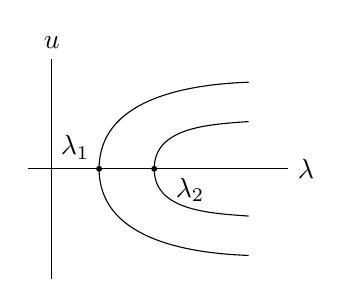
\begin{tikzpicture}
\draw (-0.3,0) -- (3,0);
\draw (0,-1.4) -- (0,1.4);
\draw (0.6,0) to [out=90, in=182] (2.5,1.1);
\draw (0.6,0) to [out=-90, in=-182] (2.5,-1.1);
\draw (1.3,0) to [out=90, in=184] (2.5,0.6);
\draw (1.3,0) to [out=-90, in=-184] (2.5,-0.6);
\node[anchor=south east] at (0.6,0) {$\lambda_1$};
\node[anchor=north west] at (1.45,0) {$\lambda_2$};
\draw[fill=black] (0.6,0) circle (0.03);
\draw[fill=black] (1.3,0) circle (0.03);
\node[anchor=west] at (3,0) {$\lambda$};
\node[anchor=south] at (0,1.4) {$u$};
\end{tikzpicture}
}
\qquad\qquad\qquad\qquad
\subfloat[][]
{
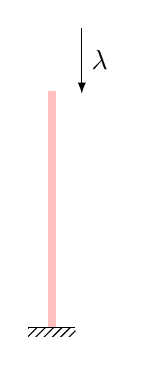
\begin{tikzpicture}
\draw (-0.3,0) -- (0.3,0);
\draw[pink,line width=3] (0,0) -- (0,3);
\pattern [pattern=north east lines] (-0.3,0) -- (-0.3,-0.12) -- (0.3,-0.12) -- (0.3,0);
%\draw[lime,line width=3] plot file {../euler/data3.dat};
\draw[violet,line width=3] plot file {../euler/data.dat};
\draw [-latex] (0.380277,3.8) -- (0.380277,2.970075);
\node[anchor=west] at (0.380277,3.4) {$\lambda$};
\end{tikzpicture}
}

\caption{(a) Schematic representation of the bifurcation diagram. (b) Buckled configuration of Euler beam calculated using Koiter asymptotic analysis.}
\label{fig:euler-beam}
\end{figure}

\subsection{Application of Koiter asymptotic analysis}

We choose $\dot w_0=v_c$. After some computation one finds that $F''(u,\lambda)vwz=\lambda(v\sin u,w)$. Then $F''_c=0$. From equation~\eqref{eqn:lambda-dot} it follows that $\dot\lambda_0=0$. Moreover from equation~\eqref{eqn:w-ddot} we have $F'c\ddot w_0=0$, so we choose $\ddot w_0=v_c$. From equation~\eqref{eqn:labda-ddot}
\[
\ddot\lambda_0=-\frac{F_c'''v_c^4}{3\hat F_c'v_c^2}=\frac{\lambda_c\int_0^L\sin\left(\frac{\pi x}{2L}\right)^4dx}{3\int_0^L\sin\left(\frac{\pi x}{2L}\right)^2dx}=\frac{\pi^2EI}{16L^2}.
\]
So we approximate the buckling path as
\[
u(t)=\left(t+\frac{t^2}{2}\right)\sin\left(\frac{\pi x}{2L}\right)+\mathscr{O}(t^3)\quad\text{and}\quad \lambda(t)=\left(1+\frac{t^2}{8}\right)\frac{\pi^2EI}{4L^2}+\mathscr{O}(t^3)
\]
The result of this analysis are in Figure~\ref{fig:euler-beam} (b).

\section{Buckling of hyperelastic continuous bodies}
\label{sec:body}

In this Section we describe our attempts, far to be complete, to apply the general theory of elastic buckling developed in Section~\ref{sec:general-buckling} to nonlinear hyperelastic continuous bodies, limiting ourself to the Green--Kirchhoff constitutive theory.

\subsection{The theory of nonlinear hyperelastic materials}

We start with a brief introduction to the theory of nonlinear hyperelastic materials. The thermomechanical foundations can be found in~\cite{gurtin-anand-fried}. The main known results concerning the well-posedness of the mathematical problems connected to this theory are collected in~\cite{ciarlet}.

\paragraph{Reference configuration and deformed configuration} Let $\Omega$ be an open bounded subset of $\mathbb{R}^2$, with Lipschitz boundary. Consider an elastic body whose reference configuration is $\Omega$. A deformed configuration of the body is described by the placement $p\colon\Omega\to\mathbb{R}^2$, where $p(x)$ is the position occupied by material point initially at $x$. The configuration of the body can be equivalently described by the displacement defined by $u(x)=p(x)-x$. We assume $u\in W^{2,p}(\Omega)^2$ for some $p\in(2,\infty)$.

\begin{rmk}
With that choice of $p$ the space $W^{2,p}(\Omega)^2$ is a reflexive Banach space.
\end{rmk}

\paragraph{Dirichlet boundary conditions} Let $\Gamma_D$ be a relatively open subset of $\partial\Omega$ with strictly positive Hausdorff measure. Suppose that the body is constrained so that $u(x)=0$ in $\Gamma_D$. We introduce the space
\[
V=\{v\in W^{2,p}(\Omega)^2\;|\;\text{$v=0$ in $\Gamma_D$ in the sense of trace}\}.
\]
Then the descriptor of the configuration of the body is any $u\in V$. The case $u=0$ correspond to the reference configuration.

\paragraph{Local measures of strain} The first local measure of strain that we consider is the deformation gradient is defined as $F=Du=I+H$ where $H=Du$. Another local measure of strain which is rotational invariant is the Green--St. Venant strain tensor defined as
\[
E=\frac{F^TF-I}{2}=\frac{H+H^T+H^TH}{2}.
\] 

\paragraph{Elastic energy density} The basic assumption of hyperelasticity is that the free (or elastic) energy density $W$ depends locally on the strain through a constitutive relation. Assuming the material to be homogeneous on isotropic, this means that pointwise in $\Omega$ should hold a relation of the form
\[
W(x)=\hat{W}(F(x))=\overline{W}(E(x))
\]
where $\hat{W}\colon\text{Lin}\to\mathbb{R}$ and $\overline{W}\colon\text{Sym}\to\mathbb{R}$. In what follows we will limit ourself to the Green--Kirchhoff constitutive theory (see~\cite{truesdell-noll}) which is based on the choice
\[
\overline{W}(E)=\frac{\gamma}{2}(\tr E)^2+\mu|E|^2,
\]
where $\gamma$ and $\mu$ are positive constants. This constitutive model describes well the behavior of steel in the presence of not too large deformations.

\begin{rmk}
The corresponding function $\hat{W}$ is
\[
\hat{W}(F)=\frac{\gamma}{8}\left(|F|^2-2\right)^2+\frac{\mu}{4}\left|F^TF-I\right|^2.
\]
%We also report below its gradient and hessian because they will be useful later.
%\begin{gather}
%\nabla \hat W(F)=\lambda\frac{|F|^2-2}{2}F+\mu(FF^TF-F),\nonumber\\
%\begin{split}
%D^2\hat W(F)KH=\lambda&\left((F\cdot H)(F\cdot K)+\frac{|F|^2-2}{2}K\cdot H\right)+\\
%&+\mu\left((KF^T)\cdot(HF^T)+(K^TF)\cdot(F^TH)+(F^TK)\cdot(F^TH)-K\cdot H\right).
%\label{eqn:D2W}
%\end{split}
%\end{gather}
\end{rmk}

\paragraph{Elastic energy of the body} The total elastic energy associated to a displacement $u\in V$ is obtained by integrating the elastic energy density over the whole body:
\[
\Phi(u)=\int_\Omega\hat W(I+Du)d\mathscr{L}=\int_\Omega\overline W\left(\frac{Du+(Du)^T+(Du)^TDu}{2}\right)d\mathscr{L}.
\]
Using that the embedding of $W^{1,p}(\Omega)$ into $C^0(\overline\Omega)$ is continuous for $p>2$, we can easily see that $\Phi\in C^\infty(V)$.

\paragraph{Energy of the loads} Suppose that on $\Gamma_N\subset\partial\Omega$, relatively open and disjoint from $\Gamma_D$, acts a traction $h\in L^{p'}(\Gamma_N)^2$. Then the energy associated to that load is
\[
-fu=-\int_{\Gamma_N}h\cdot ud\mathscr{H},\qquad\text{$f\in V'$}.
\]

\paragraph{Total energy of the body} The total energy is given by
\[
\Pi(u,\lambda)=\Phi(u)-\lambda fu,
\]
where we have introduced the multiplicative parameter $\lambda\in\mathbb{R}$ that represent the intensity of the traction. It is clear that $\Pi\in C^\infty(V\times\mathbb{R})$.

\paragraph{The equilibrium equation} We now formally show that the equilibrium equation associated to the energy $\Pi$ corresponds to the weak form of the local balance of forces of continuum solid mechanics. Indeed we have that
\[
F(u,\lambda)v=\Pi(u,\lambda)v=\int_\Omega \nabla\hat{W}(I+Du)\cdot Dvd\mathscr{L}-\lambda\int_{\Gamma_N}h\cdot vd\mathscr{H},
\]
and by formally applying Green's theorem, we find that the strong form of the equilibrium equation $F(u,\lambda)=0$ is
\[
\begin{cases}
\diver(\nabla \hat W(I+Du))=0 & \text{in $\Omega$} \\
u=0 & \text{in $\Gamma_D$} \\
\nabla \hat W(I+Du)\nu=\lambda h & \text{in $\Gamma_N$}.
\end{cases}
\]
This is indeed the local balance of forces: we recognize the Piola stress tensor $S=\nabla \hat{W}(F)$.

\begin{rmk}
\label{rmk:open-problems}
In~\cite{ciarlet} is proved an existence theorem for the equilibrium problem valid for small loads based on the Inverse Function Theorem. This result is not directly applicable to the boundary problem we are considering because it requires that displacements boundary conditions are imposed on the whole boundary. As pointed out in~\cite{open-problems}, there are no existence theorems valid for mixed displacement and traction boundary-value problems based on an analogous technique yet. The theorems proved in~\cite{ball-convexity} cover also this case but they actually establish the existence of energy minimizers. Since it is not fully understood if these minimizers are also solutions to the weak form of the equilibrium equation, these results are not useful for our analysis.
\end{rmk}

\subsection{On the applicability of the local bifurcation theorem}

To verify the hypotheses of Theorem~\ref{thm:main} we would first like to prove the existence of a fundamental path of class $C^2$ passing thought a critical point. If this were true then hypotheses (i), (iv), (v) and (vi) would be immediately satisfied. Unfortunately, to establish this result we would first have to overcome the difficulties highlighted in the Remark~\ref{rmk:open-problems}, and this is clearly beyond our capabilities.

Assuming that this first issue has been resolved, the validity of hypotheses (ii) and (iii) would still remain to be established. We do not deal with hypothesis (iii) because it should be discussed case-by-case: for example we expect that it does not hold when the reference configuration $\Omega$ has too much symmetries. Let us focus instead on hypothesis (ii). That $F_c'$ is self-adjoint was pointed out in Remark~\ref{rmk:adj}. Then we would have liked to prove that $F'(u,\lambda)$ has closed range for every $u\in V$ and $\lambda\in\mathbb{R}$. The closest result we were able to obtain is the following.
%We start with the following technical lemma.
%\begin{lemma}
%For all $u\in V$ and $\lambda\in\mathbb{R}$ the operator $F'(u,\lambda)\in\mathscr{L}(V,V')$ is coercive, i.e., there exists $\alpha>0$ such that $F'(u,\lambda)v^2\ge\alpha\norm{v}_V^4$ for all $v\in V$.
%\end{lemma}
%\begin{proof}[Sketch of the proof]
%By using~\eqref{eqn:D2W} and Young inequality can be easily shown that
%\[
%D^2\hat W(F)H^2\ge\text{c}|H|^4\quad\text{for all $H\in\text{Lin}$},
%\]
%where $c$ is a positive constant. Then
%\[
%F'(u,\lambda)v^2=\int_\Omega D^2\hat{W}(I+Du)(Dv)^2d\mathscr{L}\ge c|\Omega|\norm{Dv}_{L^4}^4.
%\]
%By Poincarè inequality there exists $C>0$ such that $\norm{u}_{L^4}\le\norm{Du}_{L^4}$ and the thesis follows.
%\end{proof}
%
%We know prove that $F'(u,\lambda)$ has closed range. Since we know also that $F'(u,\lambda)=\Pi''(u,\lambda)$ is self-adjoint, this result will allow us to apply Proposition~\ref{prop:range-adj}.
\begin{lemma}
Let $u\in V$ and $\lambda\in\mathbb{R}$ and assume that $F'(u,\lambda)\in\mathscr{L}(V,V')$ is coercive, i.e., there exists $\alpha>0$ such that $F'(u,\lambda)v^2\ge\alpha\norm{v}_V^\beta$ for all $v\in V$, where $\alpha>0$ and $\beta>1$. Then $F'(u,\lambda)\in\mathscr{L}(V,V')$ has closed range.
\end{lemma}
\begin{proof}
Call $L=F'(u,\lambda)$. Let $\{f_n\}\subset R(L)$, so $f_n=Lv_n$ for some $\{v_n\}\subset V$. Assume that $f_n\to f$ in $V'$. We have to show that there exists $v\in V$ such that $f=Lv$.

Now from hypothesis
\[
\alpha\norm{v_n-v_m}_V^\beta\le L(v_n-v_m)^2=\dual{f_n-f_m,v_n-v_m}\le\norm{f_n-f_m}_{V'}\norm{v_n-v_m}_V. 
\]
Then
\[
\alpha\norm{v_n-v_m}_V^{\beta-1}\le\norm{f_n-f_m}_{V'}.
\]
Since $\{f_n\}$ is a Cauchy sequence, also $\{v_n\}$ is a Cauchy sequence. Then $v_n\to v$ in $V$ to some $v$. By continuity $f=Lv$.
\end{proof}

\subsection{Finite element implementation of Koiter asymptotic analysis}

If we formally apply the Finite Element Method to the model of hyperelastic continuous bodies we get a \emph{new} finite dimensional model which is still included in the general theory of Section~\ref{sec:general-buckling}. Clearly the difficulties that we encounter in the original infinite dimensional problem now disappear.

We now outline the application Koiter asymptotic analysis to the discretized finite element model. We will not deal with establishing the convergence of the method nor will we study the relationship between the discretized model and the original continuous one. The main ideas are based on~\cite{casciaro}.

The MATLAB implementation is available at~\url{https://github.com/bernardo-ardini/dynamical-systems-project.git}.

\paragraph{Finite element approximation} Suppose $\Omega$ be polygonal and let $\mathscr{T}_h$ be a triangulation of it. We approximate the space $V$ with the continuous $\mathbb{P}_1$ finite element space $V_h$ of piecewise linear function on $\mathscr{T}_h$.

\paragraph{Determination of the fundamental path} In principle to determine numerically the fundamental path one should solve a nonlinear equation. This is usually done with Newton--Raphson method. Anyway, since the effect of nonlinearities can be neglected before buckling occurs, we can determine the fundamental path by a linear analysis. In particular first suppose that $u^*$ is linear in $\lambda$ so, $u^*(\lambda)=\lambda\hat u^*_0$. Then we linearize the equilibrium equation
\[
F(\lambda\hat u^*_0,\lambda)=0,
\]
obtaining
\[
F_0+\lambda F'_0\hat u^*_0+\lambda\hat F_0=0\iff \Phi''_0\hat u^*_0=f.
\]
In the finite element discretization this reduces to the solution of a linear system.

\paragraph{Determination of the critical load} To determine the critical load along the fundamental path one should solve the nonlinear eigenvalue problem
\[
F'(\lambda\hat u^*_0,\lambda)v=0,
\]
for $v\in V$ and $\lambda\in\mathbb{R}$. By linearization this becomes
\[
(F'_0+\lambda F''_0\hat u^*_0+\lambda\hat F'_0)v=0\iff\Phi''_0v=-\lambda(\Phi'''_0\hat u^*_0)v,
\]
which is a generalized linear eigenvalue problem that can be easily solved numerically. The smallest eigenvalue is the critical load $\lambda_c$. In the examples we will show the interspace has dimension one. Let $v_c$ an eigenvector. Once $\lambda_c$ has been determined we have also $u_c=\lambda_c\hat u^*_0$.

\paragraph{Second order approximation of the buckling path} By applying the formulas of Subsection~\ref{subsec:koiter} we can approximate the buckling path up to second order.

\paragraph{Some examples} In the figures below are reported some examples. On the left is reported the body in its reference configuration. In the center is reported the body in the critical configuration. On the right is the second order approximation of an equilibrium configuration along the buckling path.

\begin{figure}[p]
\includegraphics[width=\textwidth]{../fem/examples/beam.pdf}
\caption{Beam under a vertical load uniformly distributed on the top.}
\end{figure}
\begin{figure}[p]
\includegraphics[width=\textwidth]{../fem/examples/halfring.pdf}
\caption{Half ring under uniform pressure on the outer boundary.}
\end{figure}
\begin{figure}[p]
\includegraphics[width=\textwidth]{../fem/examples/box.pdf}
\caption{Box structure under a vertical load uniformly distributed on the top.}
\end{figure}
\begin{figure}[p]
\includegraphics[width=\textwidth]{../fem/examples/roundarch.pdf}
\caption{Round arch under uniform pressure on the top.}
\end{figure}

\newpage
\nocite{antman}
\nocite{brezis}
\nocite{evans}
\printbibliography

\end{document}
